% !TEX TS-program = xelatex
% !TEX encoding = UTF-8

\documentclass[12pt]{article}

\usepackage{fontspec} % Font selection for XeLaTeX; see fontspec.pdf for documentation
\defaultfontfeatures{Mapping=tex-text} % to support TeX conventions like ``---''
\usepackage{xunicode} % Unicode support for LaTeX character names (accents, European chars, etc)
\usepackage{xltxtra} % Extra customizations for XeLaTeX

\usepackage{geometry} % See geometry.pdf to learn the layout options. There are lots.
\geometry{a4paper, left=25mm, right=25mm, top=25mm, bottom=25mm} % or letterpaper (US) or a5paper or....
\usepackage[parfill]{parskip} % Activate to begin paragraphs with an empty line rather than an indent

\usepackage{graphicx} % support the \includegraphics command and options

\usepackage{listings}
\lstset{basicstyle=\ttfamily,columns=fullflexible,keepspaces=true}

%%%%%%%%%%%%%%%%%%%%%%%%%%%%%%%%%%%%%%%%%%%%%%%%%%

\title{Report 5: Memory}
\author{Dinh Ngoc Tu}

\begin{document}
\maketitle

%%%%%%%%%%%%%%%%%%%%%%%%%%%%%%%%%%%%%%%%%%%%%%%%%%

\section{Implementation}

The program runs the kernel on every pixel of the image. Each thread looks for the pixels around it to perform the convolution with the Gaussian kernel:

\begin{lstlisting}[breaklines]
int row = blockIdx.y * blockDim.y + threadIdx.y;
int col = blockIdx.x * blockDim.x + threadIdx.x;
if (row >= height || col >= width) {
    return;
}
long i = row * width + col; // position in image pixel stream
unsigned char kernel[7][7] = { // [r][c]
    { 0, 0, 1, 2, 1, 0, 0 },
    { 0, 3, 13, 22, 13, 3, 0 },
    { 1, 13, 59, 97, 59, 13, 1 },
    { 2, 22, 97, 159, 97, 22, 2 },
    { 1, 13, 59, 97, 59, 13, 1 },
    { 0, 3, 13, 22, 13, 3, 0 },
    { 0, 0, 1, 2, 1, 0, 0 },
};
long sum = 0;
long acc = 0; // sum accumulator
for (int v = 0; v < 7; v++) { // r
    for (int u = 0; u < 7; u++) { // c
        int p = col + u - 3;
        int q = row + v - 3;
        if (p < 0 || p >= width || q < 0 || q >= height) {
        } else {
            long j = q * width + p;
            int gray = ((int)input[j].x + input[j].y + input[j].z) / 3;
            acc += gray * kernel[v][u];
            sum += kernel[v][u];
        }
    }
}
output[i].x = output[i].y = output[i].z = (unsigned char)(acc / sum);
\end{lstlisting}

Shared memory is implemented by declaring a shared memory section, then initializing it in the first thread of a block:

\begin{lstlisting}[breaklines]
__shared__ int CKERNEL[7][7];
__global__ void labwork5sm(uchar3 * __restrict__ input, uchar3 * __restrict__ output, long pixelCount, int width, int height) {
    if (threadIdx.x == 0 && threadIdx.y == 0) {
        int kernel[7][7] = {
            { 0, 0, 1, 2, 1, 0, 0 },
            { 0, 3, 13, 22, 13, 3, 0 },
            { 1, 13, 59, 97, 59, 13, 1 },
            { 2, 22, 97, 159, 97, 22, 2 },
            { 1, 13, 59, 97, 59, 13, 1 },
            { 0, 3, 13, 22, 13, 3, 0 },
            { 0, 0, 1, 2, 1, 0, 0 },
        };
        for (int j = 0; j < 7; j++) {
            for (int i = 0; i < 7; i++) {
                CKERNEL[j][i] = kernel[j][i];
            }
        }
    }
    __syncthreads();
    ...
}
\end{lstlisting}

%%%%%%%%%%%%%%%%%%%%%%%%%%%%%%%%%%%%%%%%%%%%%%%%%%

\section{Speedup}

The speedup is as follows:

\begin{figure}[h]
    \centering
    \caption{Speedup with CUDA}
    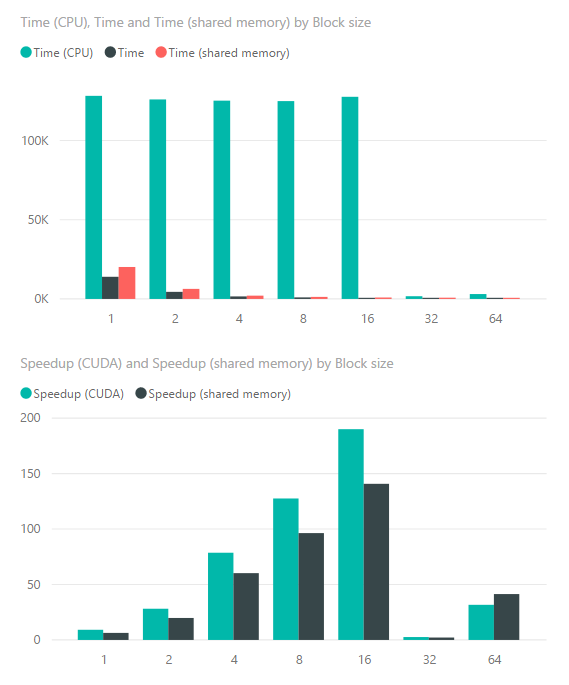
\includegraphics{pics/lw5.png}
\end{figure}

The CPU implementation has a constant speed until a blocksize of 32, which significantly reduces the program run time.
As a result, the CUDA program gains more and more speedup until a blocksize of 16, but becomes insignificantly faster at 32.
At blocksize 64, the GPU implementation again speeds up significantly, giving 31x-41x speedup over the CPU implementation at the same blocksize.
Overall, at the best configurations for each implementation, GPU gives a 17x-23x acceleration over CPU.

%%%%%%%%%%%%%%%%%%%%%%%%%%%%%%%%%%%%%%%%%%%%%%%%%%

\end{document}